\chapter{Introduction}\label{chap:introduction}

This report covers the first lab of the Security Insider Lab, which has four tasks: networking basics, monitoring tools, network attacks and defense, and machine learning for attack detection. Table~\ref{tab:split} shows how we divided the work. This chapter covers Task~1 and the background that the later chapters build on. Chapters~\ref{chap:methods} and~\ref{chap:results} turn to Task~2 and show these ideas in real packet captures. Chapter~\ref{chap:attacks} covers attacks and defenses (Task~3), Chapter~\ref{chap:ml} covers machine learning (Task~4), and Chapter~\ref{chap:discussion} brings the results together.

\begin{table}[ht]
	\centering
	\begin{tabular}{@{}lll@{}}
		\toprule
		Task & Topic & Responsible \\
		\midrule
		1 & Networking basics & Aayush Kapoor \\
		2 & Monitoring with Wireshark & Justlyn K.\ Johnson \\
		3 & Network attacks and defense & Aayush Kapoor \\
		4 & Machine learning for detection & Justlyn K.\ Johnson \\
		\bottomrule
	\end{tabular}
	\caption{Division of work in the group.}
	\label{tab:split}
\end{table}

\section{The TCP/IP Stack}\label{sec:stack}

Sending data across the world involves many separate jobs: deciding what to send, getting it there reliably, finding a route and pushing signals through a cable or over Wi-Fi. The TCP/IP stack splits these jobs into four layers (Table~\ref{tab:layers}), and each layer only talks to its direct neighbors. The OSI model describes the same idea with seven layers and is mostly used for teaching; TCP/IP is what the Internet actually runs on.

\begin{table}[ht]
	\centering
	\small
	\begin{tabular}{@{}llll@{}}
		\toprule
		Layer & Question it answers & Examples & Data unit \\
		\midrule
		Application & What is being said? & HTTP, DNS, TLS & message \\
		Transport & Which program gets it? & TCP, UDP (ports) & segment / datagram \\
		Internet & Which machine, which route? & IP, ICMP (IP addresses) & packet \\
		Link & How to cross this one hop? & Ethernet, Wi-Fi (MAC addresses) & frame \\
		\bottomrule
	\end{tabular}
	\caption{The four TCP/IP layers.}
	\label{tab:layers}
\end{table}

Think of sending a letter: the text is the data, the envelope with the address is the IP header, and the postman's bag is the frame. Every layer wraps the data in its own header, and the link layer also adds a trailer. This is called \emph{encapsulation} (Figure~\ref{fig:encap}). The receiver unwraps the layers in reverse order. A router in the middle only unwraps up to the Internet layer, because the destination IP address is all it needs, and then builds a new frame for the next hop. Only the final host passes the data up to the application. Chapter~\ref{chap:results} shows this nesting in a captured packet.

\begin{figure}[ht]
	\centering
	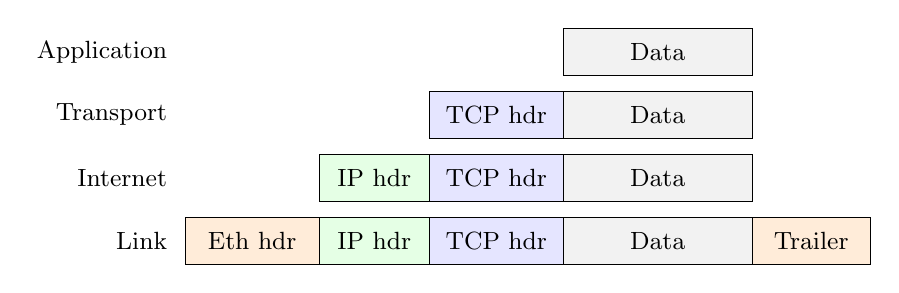
\begin{tikzpicture}[font=\small, x=1cm, y=1cm]
		\tikzset{b/.style={draw, minimum height=0.6cm, inner sep=2pt, anchor=west}}
		\node[anchor=east] at (-0.1,0) {Application};
		\node[anchor=east] at (-0.1,-0.8) {Transport};
		\node[anchor=east] at (-0.1,-1.6) {Internet};
		\node[anchor=east] at (-0.1,-2.4) {Link};
		\node[b, minimum width=2.4cm, fill=gray!10] at (4.8,0) {Data};
		\node[b, minimum width=1.7cm, fill=blue!10] at (3.1,-0.8) {TCP hdr};
		\node[b, minimum width=2.4cm, fill=gray!10] at (4.8,-0.8) {Data};
		\node[b, minimum width=1.4cm, fill=green!10] at (1.7,-1.6) {IP hdr};
		\node[b, minimum width=1.7cm, fill=blue!10] at (3.1,-1.6) {TCP hdr};
		\node[b, minimum width=2.4cm, fill=gray!10] at (4.8,-1.6) {Data};
		\node[b, minimum width=1.7cm, fill=orange!15] at (0,-2.4) {Eth hdr};
		\node[b, minimum width=1.4cm, fill=green!10] at (1.7,-2.4) {IP hdr};
		\node[b, minimum width=1.7cm, fill=blue!10] at (3.1,-2.4) {TCP hdr};
		\node[b, minimum width=2.4cm, fill=gray!10] at (4.8,-2.4) {Data};
		\node[b, minimum width=1.5cm, fill=orange!15] at (7.2,-2.4) {Trailer};
	\end{tikzpicture}
	\caption{Encapsulation: each layer adds its own header around the data from the layer above.}
	\label{fig:encap}
\end{figure}

\section{Core Network Protocols}\label{sec:protocols}

\paragraph{IP.} The Internet Protocol gives every interface an address and moves packets towards their destination on a best-effort basis: no guarantee of delivery, order or that a packet arrives only once~\cite{rfc791}. IPv4 uses 32-bit addresses (about 4.3 billion, which have run out); IPv6 uses 128-bit addresses~\cite{rfc8200}. Nothing in IP checks that a source address is genuine, so it can simply be faked. This \emph{IP spoofing} underlies several of the attacks in Task~3.

\paragraph{ICMP.} The Internet Control Message Protocol carries diagnostics and errors, such as \enquote{destination unreachable}~\cite{rfc792}. \texttt{ping} sends an echo request and waits for the reply. \texttt{traceroute} sends packets with an increasing time-to-live (TTL); every router lowers the TTL by one, and the router where it reaches zero answers with an error and thereby reveals itself. ICMPv6 does more and also handles neighbor discovery, the IPv6 replacement for ARP~\cite{rfc4443,rfc4861}.

\paragraph{TCP and UDP.} TCP provides a reliable, ordered byte stream: it numbers the data, retransmits what is lost and slows down under congestion~\cite{rfc9293}. Before any data flows, the two sides open a connection with the three-way handshake (SYN, SYN-ACK, ACK). The handshake does not check anyone's identity; it makes both sides ready and agrees on the starting sequence numbers. UDP is the opposite design: no handshake, no retransmission, almost no overhead~\cite{rfc768}. A video call prefers UDP because a late packet is useless, while online banking needs every byte in order and therefore uses TCP.

\paragraph{DNS, HTTP and TLS.} The Domain Name System translates names into IP addresses. A client asks a resolver, usually over UDP port 53, separately for IPv4 addresses (record type A) and IPv6 addresses (AAAA)~\cite{rfc1035}. HTTP is the request/response protocol of the web and runs on TCP~\cite{rfc9110}. HTTPS is HTTP inside a TLS connection, which adds confidentiality, integrity and server authentication~\cite{rfc8446}. That is why plain HTTP can be read in a capture and HTTPS cannot (Chapter~\ref{chap:results}).

\section{The Border Gateway Protocol}\label{sec:bgp}

The Internet is a collection of tens of thousands of independent networks run by ISPs, universities, companies and cloud providers. Each one is an \emph{autonomous system} (AS) with an AS number. The Border Gateway Protocol (BGP) is how these systems tell each other which IP prefixes they can reach and through which chain of ASes~\cite{rfc4271}. Each BGP router collects these announcements and, following the policy of its operator, picks a path for every destination. BGP routes \emph{between} networks, while other protocols route inside one.

BGP is a bit like airlines sharing their route maps: a passenger can reach almost any city, but only because every airline publishes where it flies. If an airline stops publishing a route, nobody sends passengers that way. Likewise, a network that stops announcing its prefixes disappears from the map.

BGP also has a trust problem. A neighbor that announces a prefix is believed unless the receiver filters it, so a network can announce address space it does not own (a \emph{hijack}) or pass on routes it should not (a \emph{route leak}). The main countermeasure is RPKI, where the owner of an address block publishes a signed statement of which AS may originate it, so that routers can reject other announcements~\cite{rfc6480}.

The Facebook outage of 4 October 2021 shows what happens when BGP goes wrong without any attacker involved. During routine backbone maintenance, a command meant to assess capacity accidentally took down the connections between Facebook's data centers~\cite{meta_outage}. Facebook's DNS servers were designed to withdraw their own BGP announcements when they cannot reach the data centers, as a safety measure. All of them did exactly that at about 15:40~UTC, and nobody could resolve \texttt{facebook.com} any more~\cite{cf_facebook}. The internal repair tools relied on the same network, so engineers had to go to the data centers in person, and the services stayed down for about six hours. BGP and DNS together decide whether a service can be found at all, however many servers are running.

\section{ISPs, IXPs and DE-CIX}\label{sec:ixp}

An Internet service provider (ISP), such as Deutsche Telekom or Vodafone, sells Internet access to homes and businesses. An Internet exchange point (IXP) is a different thing: a facility with large switches where many networks, such as ISPs, content providers and clouds, connect to exchange traffic directly. Without an IXP, two networks in the same city might send their traffic through a paid transit provider on a longer path. At an IXP, they connect to the same switch and \emph{peer}, which lowers cost and latency, keeps local traffic local and adds redundancy.

\label{sec:decix}DE-CIX in Frankfurt, Germany's largest IXP, was founded in 1995 by three German ISPs (MAZ, EUnet and XLink), who connected their networks in the back room of an old post office in the Gutleut district to reduce latency and the cost of backhaul~\cite{decix_30years}. As it grew, the switch moved into a data center in the late 1990s, and in 2013 DE-CIX introduced its Apollon platform~\cite{wiki_decix}. Today, DE-CIX runs more than 60 exchanges worldwide, and Frankfurt is the largest, with nearly 1,100 connected networks and about 48 exabytes exchanged in 2025~\cite{hessenschau_decix,techeconomy_decix}. Traffic records follow each other quickly (Table~\ref{tab:decix}); the 21.47 Tbit/s of October 2026 is more than 160\,\% above the level of early 2020~\cite{itbrief_decix}. Since these values change almost monthly, the statistics page on \texttt{de-cix.net} should be checked for the current number.

\begin{table}[ht]
	\centering
	\small
	\begin{tabular}{@{}lrl@{}}
		\toprule
		Reported & Peak at Frankfurt & Occasion \\
		\midrule
		8 July 2026 & 19.636 Tbit/s & football match (Argentina v Egypt) \cite{atv_decix} \\
		18 September 2026 & 20.02 Tbit/s & Europa League matches, first time above 20 Tbit/s \cite{techeconomy_decix} \\
		14 October 2026 & 21.47 Tbit/s & new record~\cite{itbrief_decix} \\
		\bottomrule
	\end{tabular}
	\caption{Recent traffic peaks at DE-CIX Frankfurt as reported in the press.}
	\label{tab:decix}
\end{table}
